\chapter{插讲：反常层}\label{L13}\lecturedate{2020/03/30}\sourcepage{105}
本讲介绍反常层的定义及若干性质。多数结论不在这里证明，读者可以在参考文献中查阅证明。

一般而言，反常层是同时满足\textbf{支撑条件}和\textbf{余支撑条件}的层复形。反常层之所以重要，一个原因是它们在Verdier对偶下具有良好的性质。我们先简要介绍Verdier对偶\znote{Verdier对偶是局部紧、有限维空间 $X$ 的导出范畴上的对合函子，形式为 $\mathbb D_X(\mathcal F^\bullet)=\mathrm R\mathcal Hom(\mathcal F^\bullet,\omega_X)$，其中 $\omega_X=\mathbb D_X(k_X)$ 称为对偶化复形。它把紧支上同调与普通上同调配对：$H^r_c(X,\mathcal F)^\vee\cong H^{-r}(X,\mathbb D_X\mathcal F)$。当 $X$ 是 $n$ 维光滑流形时 $\omega_X=k_X[n]$，上式即经典的Poincaré对偶；对奇异空间，对偶化复形承担了「定向」的角色。易错点是 $\mathbb D_X$ 作用于复形而非单个层。[来源：nLab "Verdier duality"，\url{https://ncatlab.org/nlab/show/Verdier+duality}（Last revised 2026-08-11；2026-11-14 访问；该条目内容较简，另见 Peters--Steenbrink《Mixed Hodge Structures》Ch. 13 §13.1）。]}：它将Poincaré对偶推广到局部紧、有限维的拓扑空间。Verdier对偶处理的是复形，更确切地说，是导出范畴中的对象。
\originalnumber{1}
\begin{definition}\label{L13S0O1}
设$X$为局部紧空间。其\textbf{维数}$\dim X$是使得对$X$上的任意阿贝尔群层$\mathcal F$均有$H_c^{n+1}(X,\mathcal F)=0$的最小非负整数$n$；若不存在这样的整数，则维数为$\infty$。这里$H_c^j(X,\cdot)$表示紧支上同调，即$\Gamma_c(X,\cdot)$的第$j$个右导出函子。
\end{definition}
\originalnumber{2}
\begin{note}[L13S0O2]
复维数为$n$的复空间，其上述维数为$2n$。
\end{note}
\section{Verdier对偶}\label{L13S1}\idx{Verdier对偶}\idx{紧支上同调}
设$X$为$n$维局部紧空间。对任意层$\mathcal F$，可以选取内射消解
\[\mathcal F\hookrightarrow\mathcal I^\bullet(\mathcal F).\]
$\mathcal I^\bullet$可能含有无穷多项，因此定义它的$n$次截断复形为以下含$n+1$项的复形：
\begin{equation}\tag{1.1}\label{L13eq11}
\begin{aligned}
{}_c\mathcal I^\bullet(\mathcal F)&:=\tau_{\le n}\mathcal I^\bullet(\mathcal F)\\
&=\bigl(\mathcal I^0(\mathcal F)\to\mathcal I^1(\mathcal F)\to\cdots\to\mathcal I^{n-1}(\mathcal F)\to\ker(\mathcal I^n(\mathcal F)\to\mathcal I^{n+1}(\mathcal F))\bigr).
\end{aligned}
\end{equation}
\sourcepage{106}
于是${}_c\mathcal I^\bullet(\mathcal F)$是$\mathcal F$的$\Gamma_c$-零调消解\idx{零调消解}。若$\mathcal F^\bullet$是有界层复形，同样可以为它构造有限长度的$\Gamma_c$-零调消解${}_c\mathcal I^\bullet(\mathcal F^\bullet)$。

设$k$为域。层复形$\mathcal F^\bullet$的\textbf{Verdier对偶}$\mathbb D_X(\mathcal F^\bullet)$，是由以下预层复形给出的层复形：对任意开集$U\subseteq X$，
\begin{equation}\tag{1.2}\label{L13eq12}
\mathbb D_X(\mathcal F^\bullet)(U):=\Hom_k^\bullet(C^\bullet(U),k),
\end{equation}
其中$C^\bullet(U)=\Gamma_c(U,{}_c\mathcal I^\bullet(\mathcal F^\bullet))$，且$\Hom^q(C^\bullet(U),k):=\Hom_k(C^{-q}(U),k)$。有如下结论。
\originalnumber{1}
\begin{proposition}[Verdier对偶]\label{L13S1O1}
设$X$为$n$维局部紧空间，$\mathcal F^\bullet$为有界层复形，则
\[\mathbb D_X(\mathcal F^\bullet)\cong\mathrm R\mathcal Hom(\mathcal F^\bullet,\mathbb D_X(k_X)),\]
其中$k_X$为$X$上茎为$k$的常值层。
\end{proposition}
更一般地，设$f:X\to Y$为两个局部紧空间之间的连续映射。考虑以下四个函子$f_!,f_*,f^!,f^{-1}$。
\begin{itemize}
\item $f_*$为直像函子，是左正合函子；若$Y=\mathrm{pt}$，则$f_*=\Gamma(\cdot)$。
\item $f_!$为真直像函子；若$Y=\mathrm{pt}$，则$f_!=\Gamma_c(\cdot)$。若$f$为真映射，则$f_!=f_*$。
\item $f^{-1}$为逆像函子，是正合函子。
\item $f^!$为非常逆像；若$f$为开嵌入，则$f^!=f^{-1}$。
\end{itemize}
按定义，$f^!$是$\mathrm Rf_!$在导出范畴中的右伴随（一般情形未必存在）。设$\mathcal G^\bullet$为$Y$上的有界层复形，则$f^!\mathcal G^\bullet$是$X$上的有界层复形。其开集$U$上的构造可写为
\begin{equation}\tag{1.3}\label{L13eq13}
U\longmapsto\Hom_Y^\bullet\bigl(f_!j_!{}_c\mathcal I^\bullet(k_U),\mathcal J^\bullet(\mathcal G^\bullet)\bigr),\qquad j:U\hookrightarrow X,
\end{equation}
其中$\mathcal J^\bullet(\mathcal G^\bullet)$为内射消解。
\originalnumber{2}
\begin{theorem}[Verdier对偶II]\label{L13S1O2}
设$f:X\to Y$为有限维局部紧空间之间的连续映射。对$Y$上的有界复形$\mathcal K^\bullet$和$X$上的有界复形$\mathcal L^\bullet$，有典范同构
\[\mathrm R\mathcal Hom_Y(\mathcal K^\bullet,\mathrm Rf_*\mathcal L^\bullet)\xrightarrow{\sim}\mathrm Rf_*\bigl(\mathrm R\mathcal Hom_X(f^{-1}\mathcal K^\bullet,\mathcal L^\bullet)\bigr).\]
对$X$上的有界复形$\mathcal F^\bullet$和$Y$上的有界复形$\mathcal G^\bullet$，有典范同构
\sourcepage{107}
\[\mathrm R\mathcal Hom_Y(\mathrm Rf_!\mathcal F^\bullet,\mathcal G^\bullet)\xrightarrow{\sim}\mathrm Rf_*\bigl(\mathrm R\mathcal Hom_X(\mathcal F^\bullet,f^!\mathcal G^\bullet)\bigr).\]
这些同构位于$D^b(Y;k)$，即$Y$上$k$-模层的有界导出范畴。此外有下图：
\begin{figure}[H]\centering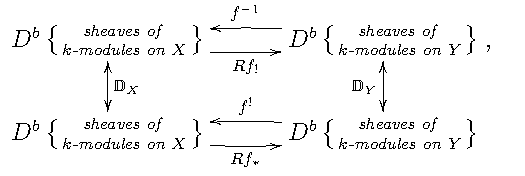
\includegraphics[width=0.4232\paperwidth]{images/L13-p107-duality.pdf}\end{figure}
它包含两个交换关系：
\[\mathrm Rf_*\circ\mathbb D_X\cong\mathbb D_Y\circ\mathrm Rf_!,\qquad \mathbb D_X\circ f^{-1}\cong f^!\circ\mathbb D_Y.\]
\end{theorem}
\originalnumber{3}
\begin{note}[L13S1O3]
域$k$可以换成具有有限同调维数的含幺交换环$R$；特别地，$R$本身具有有限长度的内射消解。例如可以取$R=\Z$。设$R\hookrightarrow\mathcal R^\bullet$为$R$的内射消解，则将\eqref{L13eq12}中的$\Hom_k^\bullet(-,k)$换成$\Hom_R^\bullet(-,\mathcal R^\bullet)$，其余构造与前面类似。
\end{note}
\section{反常层}\label{L13S2}\idx{支撑条件}\idx{余支撑条件}\idx{分层}\idx{Whitney分层}
设$k$为域，或具有有限同调维数的含幺交换环；$X$为复解析簇。代数簇$X$的一个\textbf{分层}，是将$X$分解为有限多个两两不交的部分，亦称\textbf{层}：
\[X=\coprod_{\lambda\in\Lambda}X_\lambda,\]
且满足：
\begin{enumerate}[label=(\arabic*)]
\item 每个$X_\lambda$连通、光滑，且在Zariski拓扑下局部闭；
\item 每一层的闭包都是若干层的并。
\end{enumerate}
\originalnumber{1}
\begin{definition}\label{L13S2O1}
\begin{enumerate}[label=\arabic*.]
\item 固定分层$X=\coprod_{\lambda\in\Lambda}X_\lambda$。若$X$上的$k$-模层$\mathcal F$在每层上的限制$\mathcal F|_{X_\lambda}$都是局部常值、局部有限生成的$k$-模层，则称$\mathcal F$为\textbf{$\Lambda$-可构造层}。若对某个分层$\Lambda$它是$\Lambda$-可构造层，则称它为\textbf{可构造层}。
\sourcepage{108}
\item 若层复形$\mathcal F^\bullet$的全部上同调层$\mathcal H^i(\mathcal F^\bullet)$都是可构造的，分别是$\Lambda$-可构造的，则称该复形可构造，分别为$\Lambda$-可构造。$D^b(X)$中由可构造复形、分别由$\Lambda$-可构造复形组成的满子范畴记为$D_c^b(X)$、分别记为$D_\Lambda^b(X)$。
\end{enumerate}
\end{definition}
\originalnumber{2}
\begin{note}[L13S2O2]
局部常值、局部有限生成的层也称为局部系统。注意，解析情形中的局部系统是局部常值的，而平展拓扑中的$\ell$进局部系统未必能在某个平展覆盖下平凡化。
\end{note}
\originalnumber{3}
\begin{proposition}\label{L13S2O3}
设$X,Y$为复解析簇。
\begin{enumerate}[label=(\arabic*)]
\item 导出张量积和导出$\mathcal Hom$函子都保持可构造性。
\item Verdier对偶算子$\mathbb D_X$保持可构造性。
\item 若$f:X\to Y$为态射，则$f^{-1}$和$f^!$保持可构造性。若$f$为真映射，或为复代数簇之间的态射，则$\mathrm Rf_*$和$\mathrm Rf_!$也保持可构造复形。
\end{enumerate}
\end{proposition}
设$f:X\to Y$为真映射。现在以$D_c^b(-)$代替$D^b(-)$来讨论，有如下结论。
\originalnumber{4}
\begin{theorem}\label{L13S2O4}
\begin{enumerate}[label=\arabic*.]
\item Verdier对偶算子$\mathbb D_X$是对合，即$\mathbb D_X^2\cong\mathrm{Id}$。
\item \textbf{真基变换：}对任意下列Cartesian图，其中底边映射记为$g:Y'\to Y$（顶边为$f:X\to Y$，右边为$f':X'\to X$，左边为$g':X'\to Y'$），
\begin{figure}[H]\centering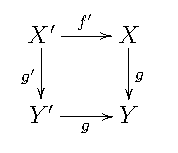
\includegraphics[width=0.1434\paperwidth]{images/L13-p108-basechange.pdf}\end{figure}
有函子同构
\[f^{-1}\circ\mathrm Rg_!\cong\mathrm Rg'_!\circ f'^{-1}.\]
\item \textbf{投影公式：}有函子同构
\[(\mathrm Rf_!(-))\otimes^{\mathrm L}(-)\cong\mathrm Rf_!\bigl((- )\otimes^{\mathrm L}f^{-1}(-)\bigr),\]
其中$\otimes^{\mathrm L}$表示导出张量积。
\sourcepage{109}
\item 有函子同构
\[\mathrm R\mathcal Hom(f^{-1}(-),f^!(-))\cong f^!\mathrm R\mathcal Hom(-,-).\]
\item \textbf{开闭三角：}设$U\hookrightarrow X$为Zariski开嵌入，$Z=X\setminus U$；令$j:U\to X$、$i:Z\to X$分别为开、闭嵌入。则在$D^b(X)$中有函子性的正合三角
\[i_!i^!\to\mathrm{Id}\to\mathrm Rj_*j^*\xrightarrow{[1]},\qquad j_!j^!\to\mathrm{Id}\to i_*i^*\xrightarrow{[1]}.\]
\end{enumerate}
\end{theorem}
\originalnumber{5}
\begin{definition}\label{L13S2O5}
固定分层$X=\coprod_{\lambda\in\Lambda}X_\lambda$，使$\mathbb D_X$保持$D_\Lambda^b(X)$，例如可以取Whitney分层。若$\Lambda$-可构造层复形$\mathcal F^\bullet$满足下列两个条件，则称它是相对于$\Lambda$的\textbf{反常层}\znote{反常层由 Beilinson--Bernstein--Deligne 在研究六函子形式时引入，perverse 一词只表明其截断位置与通常层复形相反；它并不是层，而是满足支撑条件与余支撑条件的可构造复形。两个条件把上同调挤进与分层维数匹配的窄区间：在复维数 $d$ 的层 $X_\lambda$ 上只允许 $j\le-d$ 的 $\mathcal H^j$，余支撑条件则对偶地限制 $i_x^!\mathcal F^\bullet$ 的非零范围。关键结论是 $\operatorname{Perv}(X)$ 为阿贝尔范畴，而 $D_c^b(X)$ 不是，因此反常层上可以谈论子对象、商对象与单性。[来源：nLab "perverse sheaf"，\url{https://ncatlab.org/nlab/show/perverse+sheaf}（Last revised 2026-10-16；2026-11-14 访问）。]}：
\[\begin{cases}
\mathcal H^j(\mathcal F^\bullet)_x=0,&x\in X_\lambda,\ j>-\dim_{\C}X_\lambda,\\
\mathcal H^j(i_x^!\mathcal F^\bullet)=0,&x\in X_\lambda,\ j<\dim_{\C}X_\lambda.
\end{cases}\]
这里$i_x:\{x\}\hookrightarrow X$。若$\mathcal F^\bullet$相对于某个分层$\Lambda$为反常层，就称它为反常层。$D_c^b(X)$中由$k$-模反常层组成的满子范畴记为$\operatorname{Perv}(X)$。
\end{definition}
\originalnumber{6}
\begin{note}[L13S2O6]
\textbf{Whitney分层}是满足Whitney条件的分层：设$X_\mu\subseteq\overline{X_\lambda}$，有点列$\{a_n\}\subseteq X_\mu$、$\{b_n\}\subseteq X_\lambda$，两者都趋于同一点$c\in X_\mu$。若连接$a_n,b_n$的割线以及$X_\lambda$在$b_n$处的切空间分别存在极限，则割线的极限包含于切空间的极限中。

每个复代数簇都具有Whitney分层；并且任意分层都可以细化为Whitney分层。
\end{note}
\originalnumber{7}
\begin{lemma}\label{L13S2O7}
设$k$为特征零的域，$\mathcal F^\bullet$为有界可构造$k$-模层复形。它为反常层，当且仅当满足下列两条件：
\[\begin{aligned}
\dim_{\C}\operatorname{Supp}\mathcal H^j(\mathcal F^\bullet)&\le-j&&\text{（支撑条件）},\\
\dim_{\C}\operatorname{Supp}\mathcal H^j(\mathbb D_X(\mathcal F^\bullet))&\le-j&&\text{（余支撑条件）}.
\end{aligned}\]
特别地，$\mathcal F^\bullet$为反常层，当且仅当其Verdier对偶$\mathbb D_X(\mathcal F^\bullet)$为反常层；反常性不依赖于所选的分层。
\end{lemma}
\sourcepage{110}
定义反常层的另一种方式，是把$\operatorname{Perv}(X)$看作三角范畴$D_c^b(X)$的某个截断结构的\textbf{心}。以$[n]$表示平移函子，约定$(\mathcal F^\bullet[n])^q=\mathcal F^{n+q}$。
\originalnumber{8}
\begin{definition}\label{L13S2O8}\idx{t结构}\idx{心（t结构）}
三角范畴$D$上的\textbf{截断结构}，简称\textbf{$t$结构}\znote{$t$结构是对三角范畴中「截断」的公理化：一对满子范畴 $(D^{\le0},D^{\ge0})$ 保证每个对象 $S$ 都同构意义下唯一地落入三角 $A\to S\to B\xrightarrow{[1]}$，其中 $A\in D^{\le0}$、$B\in D^{\ge1}$，于是可以定义截断函子 ${}^t\tau_{\le0}$、${}^t\tau_{\ge1}$ 与上同调函子 ${}^t\mathcal H^n$。其心 $C(D,t)=D^{\le0}\cap D^{\ge0}$ 自动是阿贝尔范畴，这是 $t$ 结构最重要的性质。阿贝尔范畴的导出范畴上由 $\mathcal H^j$ 的消失范围给出标准 $t$ 结构；本讲后文要说明 $D_c^b(X)$ 上还存在反常 $t$ 结构，其心正是 $\operatorname{Perv}(X)$。[来源：nLab "t-structure"，\url{https://ncatlab.org/nlab/show/t-structure}（Last revised 2023-04-20；2026-11-14 访问）。]}，是一对满子范畴$(D^{\le0},D^{\ge0})$，满足：
\begin{enumerate}[label=(\roman*)]
\item 令$D^{\le n}:=D^{\le0}[-n]$、$D^{\ge n}:=D^{\ge0}[-n]$，则$\Hom(D^{\le0},D^{\ge1})=0$。
\item $D^{\le-1}\subseteq D^{\le0}$且$D^{\ge1}\subseteq D^{\ge0}$。
\item 任意$S\in\operatorname{ob}(D)$都属于一个区别三角
\begin{equation}\tag{2.1}\label{L13eq21}A\to S\to B\xrightarrow{[1]},\end{equation}
其中$A\in D^{\le0}$、$B\in D^{\ge1}$。
\end{enumerate}
给定$t$结构的\textbf{心}，亦称核心，定义为$C(D,t):=D^{\le0}\cap D^{\ge0}$。
\end{definition}
\originalnumber{9}
\begin{example}\label{L13S2O9}
阿贝尔范畴$\mathcal A$的导出范畴$D(\mathcal A)$上有一个自然的$t$结构：
\[\begin{aligned}
\operatorname{ob}(D^{\le0})&:=\{\mathcal G^\bullet\in\operatorname{ob}(D(\mathcal A))\mid\mathcal H^j(\mathcal G^\bullet)=0,\ \forall j>0\},\\
\operatorname{ob}(D^{\ge0})&:=\{\mathcal G^\bullet\in\operatorname{ob}(D(\mathcal A))\mid\mathcal H^j(\mathcal G^\bullet)=0,\ \forall j<0\}.
\end{aligned}\]
该$t$结构的心等价于阿贝尔范畴$\mathcal A$。
\end{example}
由下面的\eref{引理}{L13S2O10}，\eqref{L13eq21}中的对应$S\mapsto A$、分别$S\mapsto B$给出良定义的函子，记为${}^t\tau_{\le0}$、分别记为${}^t\tau_{\ge1}$。类似地，定义
\[{}^t\tau_{\le a}:=[-a]\circ{}^t\tau_{\le0}\circ[a],\qquad {}^t\tau_{\ge b}:=[1-b]\circ{}^t\tau_{\ge1}\circ[b-1].\]
对任意$a,b\in\Z$，有典范同构${}^t\tau_{\le a}\circ{}^t\tau_{\ge b}\cong{}^t\tau_{\ge b}\circ{}^t\tau_{\le a}$。
\sourcepage{111}
\originalnumber{10}
\begin{lemma}\label{L13S2O10}
设$D$为三角范畴，考虑两个区别三角$A\to S\to B\xrightarrow{[1]}$、$A'\to S'\to B'\xrightarrow{[1]}$和$D$中的映射$g:S\to S'$。考虑下图：
\begin{figure}[H]\centering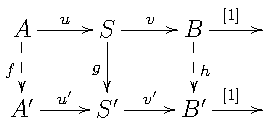
\includegraphics[width=0.2242\paperwidth]{images/L13-p111-triangles.pdf}\end{figure}
下列条件等价：
\begin{enumerate}[label=(\arabic*)]
\item 存在$f$，使第一个方块交换；
\item 存在$h$，使第二个方块交换；
\item 存在三角之间的态射$(f,g,h):(A,S,B)\to(A',S',B')$；
\item $v'\circ g\circ u=0$。
\end{enumerate}
此外，若这些条件成立，且$\Hom(A[1],B')=0$，则$f$和$h$唯一。
\end{lemma}
\originalnumber{11}
\begin{theorem}\label{L13S2O11}
给定$D$上的$t$结构$(D^{\le0},D^{\ge0})$，其心$C(D,t)$为阿贝尔范畴，且函子
\[D\longrightarrow C(D,t),\qquad S\longmapsto{}^t\tau_{\le0}\circ{}^t\tau_{\ge0}(S)\]
为上同调函子。
\end{theorem}
令${}^t\mathcal H^n(S):={}^t\tau_{\le0}\circ{}^t\tau_{\ge0}(S[n])$。
\originalnumber{12}
\begin{theorem}\label{L13S2O12}
定义$D_c^b(X)$的两个满子范畴${}^pD^{\le0}$、${}^pD^{\ge0}$如下：
\[\begin{aligned}
\operatorname{ob}({}^pD^{\le0})&:=\{\mathcal F^\bullet\in\operatorname{ob}(D_c^b(X))\mid\mathcal F^\bullet\text{满足支撑条件}\},\\
\operatorname{ob}({}^pD^{\ge0})&:=\{\mathcal F^\bullet\in\operatorname{ob}(D_c^b(X))\mid\mathcal F^\bullet\text{满足余支撑条件}\}.
\end{aligned}\]
则$({}^pD^{\le0},{}^pD^{\ge0})$是$D_c^b(X)$上的$t$结构，有时称为\textbf{反常$t$结构}。
\end{theorem}
\sourcepage{112}
\originalnumber{13}
\begin{corollary}\label{L13S2O13}
范畴$\operatorname{Perv}(X)$是阿贝尔范畴。
\end{corollary}
因此，反常层就是$D_c^b(X)$上反常$t$结构的心中的对象。对任意$\mathcal F^\bullet\in D_c^b(X)$，反常层
\[{}^p\mathcal H^n(\mathcal F^\bullet)={}^p\tau_{\le0}\circ{}^p\tau_{\ge0}(\mathcal F^\bullet[n])\]
称为$\mathcal F^\bullet$的\textbf{第$n$个反常上同调}\znote{反常上同调 ${}^p\mathcal H^n$ 与通常的上同调层 $\mathcal H^n$ 不是一回事：后者对复形逐项取上同调，前者先在反常 $t$ 结构下截断再取心，二者一般不同。由定义，$\mathcal F^\bullet$ 是反常层当且仅当 ${}^p\mathcal H^n(\mathcal F^\bullet)=0$ 对所有 $n\ne0$ 成立且 ${}^p\mathcal H^0(\mathcal F^\bullet)=\mathcal F^\bullet$。检验反常性时最容易混淆的正是这两套上同调，计算反常上同调必须始终在 $\operatorname{Perv}(X)$ 中进行。[来源：nLab "perverse sheaf"，\url{https://ncatlab.org/nlab/show/perverse+sheaf}（Last revised 2026-10-16；2026-11-14 访问）。]}。\idx{反常上同调}
\originalnumber{14}
\begin{note}[L13S2O14]
若$\mathcal F^\bullet$为反常层，则
\[{}^p\mathcal H^n(\mathcal F^\bullet)=\begin{cases}0,&n\ne0,\\\mathcal F^\bullet,&n=0.\end{cases}\]
\end{note}
设$T:D\to D'$为带有$t$结构的三角范畴之间的函子。如果$T$与平移相容，即$T(X)[1]\cong T(X[1])$，并将区别三角映为区别三角，就称$T$为\textbf{加性函子}。对这样的$T$，可以引入心之间的相关函子
% [Tutor Note: 原书 p112 称这类函子为 additive，译文照译为「加性函子」；按通行术语应称三角函子（与平移相容、把区别三角映为区别三角），这里的「加性」不含通常意义下加性函子的含义。]
\begin{equation}\tag{2.2}\label{L13eq22}
{}^tT:={}^{t'}\mathcal H^0\circ T\circ\epsilon:C(D,t)\longrightarrow C(D',t'),
\end{equation}
其中$\epsilon:C(D,t)\to D$为自然包含函子。若$T(D^{\le0})\subseteq D'^{\le0}$，则称$T$相对于$t$结构\textbf{左正合}；若$T(D^{\ge0})\subseteq D'^{\ge0}$，则称它\textbf{右正合}。若同时左、右正合，就称为\textbf{正合}。显然，若$T$相对于$t$结构正合，则${}^tT$就是$T$在心$C(D,t)$上的限制\znoteplain{这里的「左正合」「右正合」是一对\textbf{约定}，不是定理，不同学派的约定方向相反：Beilinson--Bernstein--Deligne 一系把「保 $D^{\le0}$」称为左正合，Kashiwara--Schapira 一系则把方向反过来，本讲按原书取前一种。读下文时须与此配套：$f^{-1}$ 对开嵌入、$f_*$ 对闭嵌入相对于反常 $t$ 结构正合，这里的「正合」与该约定无关，但引用他人文献中的「左/右 $t$-正合」前务必先核对其约定，否则容易读反。（上下文推断，无外部依据）}。

注意，开嵌入的$f^{-1}$和闭嵌入的$f_*$相对于反常$t$结构都是正合的。但一般而言，$f^{-1},f^!,\mathrm Rf_*,\mathrm Rf_!$虽然是加性函子，却不保持反常性。因此，为了将反常层送到反常层，可以对它们使用\eqref{L13eq22}定义的相关函子。
\section{交复形}\label{L13S3}\idx{交复形}\idx{中间延拓}
交复形\znote{交复形由 Goresky--MacPherson 为研究奇异空间的上同调而构造。想法是：先在稠密光滑开子集上给定局部系统 $\mathbb V$，再用截断 $\tau_{\le n-1}\mathrm Rj^n_*$ 逐层向高维层延拓，使延拓所得复形在每个层上恰好满足支撑条件——这正是下面递归定义的来源。所得复形平移 $[d]$ 后是反常层，称为 $\mathbb V$ 的反常延拓，其超上同调即交上同调；当 $X$ 本身光滑时它退化为普通上同调。[来源：nLab "intersection cohomology"，\url{https://ncatlab.org/nlab/show/intersection+cohomology}（Last revised 2023-05-07；2026-11-14 访问）。]}是反常层的重要例子。以下取域系数$k$。将Whitney分层中复维数不超过$i$的层合并，得到滤过
\[F_0(X)\subseteq F_1(X)\subseteq\cdots\subseteq F_m(X)=X.\]
设$\mathbb V$为稠密光滑开子集$U_1:=X\setminus F_{m-1}(X)$上的$k$-模局部系统，即局部常值、局部有限生成的层。
\sourcepage{113}
定义$U_n:=X\setminus F_{m-n}(X)$、$j^n:U_n\hookrightarrow U_{n+1}$，并令$U_{m+1}=X$。$U_1$上的$\mathbb V$所对应的\textbf{交复形}记为$IC_X^\bullet\mathbb V$，递归定义如下：
\[\begin{cases}
IC_X^\bullet\mathbb V|_{U_1}=\mathbb V,\\
IC_X^\bullet\mathbb V|_{U_{n+1}}=\tau_{\le n-1}\mathrm Rj^n_*\bigl(IC_X^\bullet\mathbb V|_{U_n}\bigr),&n=1,\ldots,m.
\end{cases}\]
这里$\tau_{\le n-1}$为通常的截断函子，与\eqref{L13eq11}类似。

设$X$为纯维数$d$的复代数簇。对$X$的正则点集中的任意稠密开子集上的局部系统$\mathbb V$，交复形的平移$IC_X^\bullet\mathbb V[d]$为反常层，称为$\mathbb V$到$X$的\textbf{反常延拓}，记为${}^p\mathbb V_X$。
\originalnumber{1}
\begin{theorem}\label{L13S3O1}
设$X$为纯$d$维、可分层的复空间，$U$为其中稠密光滑的Zariski开子集，$\mathbb V$为$U$上的$k$-模局部系统。在相差拟同构的意义下，${}^p\mathbb V_X$是$X$上唯一的$k$-模反常层，它在$U$上的限制为$\mathbb V[d]$，且不存在支撑于$X\setminus U$上的非零反常子对象或商对象。
\end{theorem}
\originalnumber{2}
\begin{corollary}\label{L13S3O2}
在$D_c^b(X)$中，有$\mathbb D_X({}^p\mathbb V_X)\cong{}^p(\mathbb V^\vee)_X$。
\end{corollary}
\eref{定理}{L13S3O1}说明，交复形具有内在意义，不应依赖于分层。下面的命题实际上给出了交复形的另一种定义。对开嵌入$j:U\to X$，有自然的函子态射$j_!\to\mathrm Rj_*$，因而定义\textbf{反常中间直像函子}
\[{}^pj_{!*}\mathcal F^\bullet:=\operatorname{Im}\bigl({}^pj_!\mathcal F^\bullet\to{}^pj_*\mathcal F^\bullet\bigr),\qquad\mathcal F^\bullet\in\operatorname{Perv}(U).\]
\originalnumber{3}
\begin{proposition}\label{L13S3O3}
设$X$为复簇，$Z\subseteq X$为等维闭子簇。令$\mathbb V$为$Z$的光滑点组成的稠密开子集$U$上的局部系统，$i:Z\hookrightarrow X$、$j:U\hookrightarrow Z$为包含映射，则
\[{}^p\mathbb V_Z:=i_*\bigl({}^pj_{!*}(\mathbb V[d_Z])\bigr),\qquad d_Z=\dim Z,\]
为反常层，且等于支撑于$Z$上的交复形$i_*IC_Z^\bullet\mathbb V[d_Z]$。特别地，$X=Z$时，${}^p\mathbb V_X$不依赖于分层。
\end{proposition}
\sourcepage{114}
由交复形得到的反常层实际上生成Grothendieck群$K_0(\operatorname{Perv}(X))$，如下定理所述。
\originalnumber{4}
\begin{theorem}\label{L13S3O4}
设$X$为复空间。若$\mathcal F^\bullet$是$X$上的反常层，且相对于$X$的某个有限分层可构造，则$\mathcal F^\bullet$具有Jordan--Hölder列，即各个相继商均为单对象的有限滤过。特别地，若$X$为复代数簇，则每个反常层都具有Jordan--Hölder列，因而$\operatorname{Perv}(X)$为Artin（满足降链条件）范畴\znoteplain{这里的「Artin」指范畴中每个对象满足子对象降链条件（Artin 条件）；该词取自已故数学家 Emil Artin 之名，与代数几何中「阿廷叠」（Artin stack）、「Artin 逼近」等术语里的 Artin 所指不同，阅读时请看条件本身而非名字。（上下文推断，无外部依据）}。

$\operatorname{Perv}(X)$中的单对象$S^\bullet$正是支撑于不可约子空间$Z\subseteq X$上的${}^p\mathbb V_Z$，其中$\mathbb V$对应于$\pi_1(U)$的一个不可约表示；$U\subseteq Z$为$S^\bullet$的适当平移局部常值的最大光滑开子集。
\end{theorem}
\needspace{5\baselineskip}\section{第13讲参考文献}\label{L13S4}
\begin{references}
\refitem{L13bibW}{W} Geordie Williamson, \emph{An illustrated guide to perverse sheaves}, lecture notes on webpage at \url{http://people.mpim-bonn.mpg.de/geordie/perverse_course/}.
\refitem{L13bibPS}{PS} Chris A. M. Peters and Joseph H. M. Steenbrink, \emph{Mixed Hodge Structures}, Springer-Verlag Berlin Heidelberg, Ch. 13 \S13.1, \S13.2.
\end{references}
